\section{Enunciado}

\hspace{1.27cm} En la \hyperref[fig1]{Figura 1} se muestra un estanque que se utiliza para monitoreo de especies marinas
endémicas de la Isla del Coco, donde se tiene un tanque cilíndrico vertical abierto en su
parte superior a la atmósfera, del cual se desea controlar el nivel del tanque manipulando
el caudal de entrada $Q_e$ ante posibles perturbaciones en el caudal de salida $Q_s$.

\begin{figure}[!h]
    \centering
    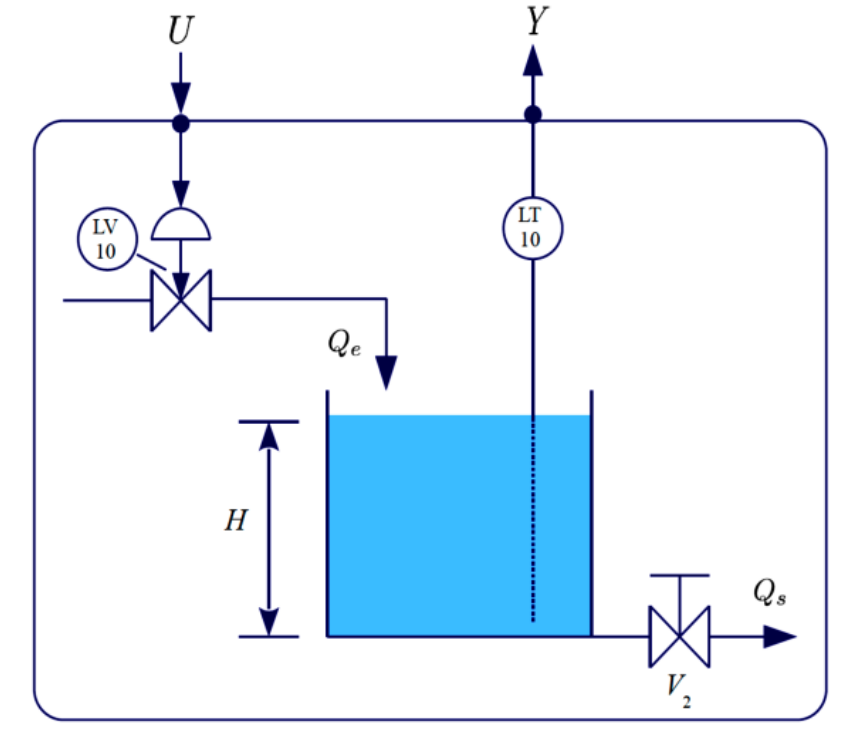
\includegraphics[width = 0.4\linewidth]{figs/fig1.png}
    \caption{Proceso Control de Nivel}
    \label{fig1}
\end{figure}

El modelo dinámico del proceso es:
\begin{align*}
    A\dv{H(t)}{t} = Q_e(t) -Q_s(t) = Q_e(t) - X _{vs} (t) K _{vs} \sqrt{\rho g H(t)}
\end{align*}
La característica estática es:
\begin{align*}
    H(t) = f (Q_e, X _{vs}) = \frac{1}{\rho g} \left( \frac{Q_e(t)}{X _{vs} (t) K _{vs}} \right) ^{2}
\end{align*}

El modelo linealizado es:
\begingroup 
\addtolength\jot{6pt} 
\begin{align*}
    h (s) = \frac{K _{1}}{ Ts + 1} q _{e} (s) &+ \frac{K _{2}}{Ts + 1} x _{vs} (s)\\
    K _{1} = \frac{2}{X _{vs0} K _{vs}} \sqrt{ \frac{H_0}{\rho g}}, \quad K _{2} =& - \frac{2 H_0}{X _{vs0}}, \quad T = \frac{2A}{X _{vs0} K _{vs}} \sqrt{ \frac{H_0}{\rho g}}
\end{align*}

\newpage
En donde:

\begin{figure}[!h]
    \centering
    \setlength\extrarowheight{3mm}
    \begin{tabular}{>{\centering\arraybackslash}p{5cm}p{5cm}>{\centering\arraybackslash}p{5cm}}
        \toprule\\[-2.5em]
        Variable/Parámetro & Descripción & Valor nominal\\
        \midrule
        $A$ & área transversal del tanque & \SI{5}{\metre\squared}\\
        $g$ & aceleración de la gravedad & \SI{9.81}{\metre\per\second\squared}\\
        $H$ & nivel de líquido en el tanque & [2.24 2.5 2.95] m\\
            & Altura máxima del tanque & \SI{3.6}{m}\\
            & Ámbito de medición del sensor & \SI{0}{m} -- \SI{3.25}{m} \\
        $Q _{e}$ & caudal de líquido de entrada & -- \\
        $Q _{s}$ & caudal de líquido de salida & -- \\
        $K _{vs}$ & constante de la válvula de salida del tanque & 0.001 \\
        $X _{vs}$ & apertura de la válvula de salida del tanque & \{0.4 0.5 0.6\} \\
        $\rho$ & densidad del líquido (agua de mar) & \SI{1027}{kg/\metre\cubed} \\
        $t$ & tiempo & s \\
        \bottomrule
    \end{tabular}
    \captionof{table}{Variables y parámetros del proceso control de nivel}
    \label{lmao}
\end{figure}

Para este sistema:

\begin{enumerate}[label=\alph*)]
    \item (5 puntos) Demuestre la obtención de la ecuación en el tiempo del modelo linealizado a
partir del modelo dinámico del sistema, utilizando el procedimiento algebraico de
linealización visto en clase, y a partir del mismo demuestre la obtención de las
respectivas funciones de transferencia.
\end{enumerate}

Utilizando la plantilla \texttt{Tarea\_1.m} de MATLAB disponible en mediación virtual, calcule 

\begin{enumerate}[label=\alph*), start=2]
    \item (5 puntos) La ganancia del transmisor de nivel $K_t$. (\SI{}{\%\metre\tothe{-1}}) de forma que la señal
realimentada esté normalizada de 0 a 100\%.
    \item (5 puntos) La constante de la válvula $K _{VC}$ (\SI{}{\metre\cubed\second\tothe{-1}\%\tothe{-1}}) de forma que la acción de control esté normalizada de 0\% a 100\%.
    \item (20 puntos) Implemente el sistema real en Simulink utilizando la ecuación del modelo
        dinámico del proceso tal como se observa en la Figura 2. %\hyperref[fig2]{Figura 2}. 
        \textbf{Debe indicar la condición inicial ($H_0$) en los parámetros del bloque Integrador.}
    \item (15 puntos) Calcule el valor de $T$, $K_1$, $K_2$ del modelo linealizado. Implemente el diagrama de bloques en Simulink del sistema tal como se observa en la Figura 3.
    \item (20 puntos) Obtenga la respuesta del sistema (obtenida en el punto c) y compárela con la del sistema linealizado (obtenida en el punto d) \textbf{en una misma gráfica} utilizando Simulink/MATLAB, cuando ambos se encuentran en el punto de operación más probable y se producen los siguientes cambios:
        \begin{enumerate}[label=\roman*.]
            \item Un cambio escalón en la señal de control de $\Delta U = -2\%$, seguido de un cambio escalón en la perturbación de $\Delta D = -0.02$.
                Considere que el sistema debe estabilizarse antes de aplicar el segundo cambio escalón.
            \item Un cambio escalón de la señal de control de $\Delta U = -10\%$, seguido de un cambio escalón en la perturbación de $\Delta D = -0.1$. Considere que el sistema debe estabilizarse antes de aplicar el segundo cambio escalón.
        \end{enumerate}
        Indique las gráficas en su solución y adjunte el archivo \texttt{.slx}.
    \item (20 puntos) A partir de la ecuación de la característica estática obtenga utilizando MATLAB
y en una misma figura, la curva estática del proceso para los tres posibles valores de la
apertura de la válvula de salida. Muestra la relación entre $m(t)$ y $c(t)$. 
\textbf{Indique en la figura el punto de operación más probable del sistema}. Presente la gráfica en su solución y comente sobre la forma de las curvas.
    \item (10 puntos) A partir de los resultados anteriores, observe la respuesta del nivel ante los
cambios en el caudal de entrada y la apertura de la válvula de salida, ¿son razonables?
Comente sobre la validez del modelo lineal cuando se producen cambios en el punto
de operación del sistema.
\end{enumerate}

